\section{Extended Study: What Survives When the Setup Changes?}\label{sec:extended}
The confirmatory study answers \Q1--\Q4 for one configuration. A reader building on it needs to know which conclusions
depend on our choices. We therefore ran a controlled study (overview in Fig.~\ref{fig:overview}, Appendix~\ref{app:ext}): starting from the test-set
configuration, each of 19 rows changes \emph{one} design choice and reruns all six methods on the same 40 objects, four
values of $r$ and the same episode seeds; four rows retrain the residuals. Four diagnostic rows (R0L, E7L, E9L, T2L) were
added after some results were seen, each frozen before it was run. Figure~\ref{fig:ctrl} reports the change in
failure rate, grip and episode time for every cell, with a paired bootstrap over objects marking changes whose 95\%
interval excludes zero (an unpaired bootstrap for E1 and E2, which draw different objects). Table~\ref{tab:changes} in the
appendix describes each change and Table~\ref{tab:controlled} gives absolute values. The study, and the analyses in
Sections~\ref{sec:map}--\ref{sec:tight}, were frozen in a protocol addendum before they were run and are exploratory.





\subsection{Findings that hold}
\finding{The unshielded residual is fragile, and the shield fixes it.} B2's failure rate moved with almost every change:
from 11.5\% in the reference to 26\% for heavier objects (E1), 30\% with a finer probe (E6), 15\% with softer pads (E8) and
14\% with a 2\,mm tolerance (S4). In every one of these rows, and in the weight-error and probe-step rows, B4g, B4t and B5
had zero failures. A finer probe is an instructive case: it brings $\Fs$ closer to the true breakaway grip, which removes
some of the hidden margin that B2 had learned to spend, so B2 fails more while the shielded methods do not notice.

\finding{The cliff holds.} Setting the shield to $r_{\max}=1.1$ (S2) lowered B5's grip by only 0.19 percentage points of the
object's weight, and $r_{\max}=1.4$ (S3) changed nothing: once any drop is assumed, the certified grip is the no-onset grip.
Removing the 1.5\,mm sensing margin (S6) or widening the tolerance to 10\,mm (S5) did not change the shielded grip at all.
Only $r_{\max}=1.0$ (S1) bought grip, $-7$ to $-9$ points, and it cost 5--7.5\% failures, as in \Q4.

\subsection{Findings that break}
\finding{A probe that fails gives the shield nothing to certify.} Our probe starts at the grip that would hold the
estimated weight at $\mu=0.3$. With slippery objects ($\mu_s\in[0.2,0.4]$, E2) the first step already slips for many
objects; with a noisier slip monitor (1.5\,mm, E3) noise alone exceeds the 2.5\,mm motion threshold on the first step. In
both cases the probe reports $\Fs=30$\,N, the maximum grip. The shield then certifies nothing: it declined on 68\% (E2) and
100\% (E3) of lifts and fell back to the slow model lift, at 21 to 31 times the object's weight in grip. This is a safe
failure, but not a gentle one, and Fig.~\ref{fig:ctrl}a shows why failure rates alone mislead here: B2's failure rate
\emph{fell} in these rows because it, too, was handed a crushing grip.

\finding{The certificate assumes friction stays static until gross slip, and that assumption can fail.} Two rows broke the
shield itself. Lifting 20\,cm instead of 10\,cm (E7) doubles the peak acceleration for the same duration; B5 then failed
38.6\% of lifts and B4g 37.8\%, every one with a certified bound of zero. Switching to kinetic friction at 5\,mm/s instead
of 2\,cm/s (E9) gave 46.9\% for both. Figure~\ref{fig:e7case} shows the mechanism. The shield sets the grip at the edge of
onset, where the demand reaches 95\% of the true static capacity at peak acceleration. At that load MuJoCo's soft contact
lets the rod creep relative to the pads, at up to 12\,mm/s in E7 (6.5\,mm/s in the reference). Our emulator decides when
friction drops by comparing the rod's velocity from the previous step with the palm's commanded velocity for the current
step; this one-step lag adds $a\,\Delta t$, about 8\,mm/s at E7's peak acceleration, to the measured relative speed. Creep
plus lag crossed the 20\,mm/s threshold, friction dropped although Coulomb's law says the rod was stuck, and the rod slid.
In the reference configuration the same quantity peaked at 10.8\,mm/s, and no shielded lift ever switched to kinetic
friction (0 of 2{,}560). The time projection was more robust in E7 (4.1\% failures), because a longer lift lowers the peak
demand instead of meeting it at the edge.

\finding{Removing the lag.} (pending)


So E7 was an artefact, but E9 exposes something real. The shield places the grip exactly at the onset boundary, where
the contact already creeps; if friction weakens during that creep, the certificate's premise (static friction until gross
slip) fails. Real contacts also move before they slide: pre-sliding displacement is part of every dynamic friction
model~\cite{canudas1995,olsson1998}, and whether friction weakens during it depends on the materials. \textbf{The practical
fix is a margin on onset}, certifying $g+a\le(1-\delta)\,gF/\Fs$ for some $\delta>0$, which our zero-margin shield did not
have. We report this as found rather than adding the fix after seeing the result.



\subsection{Training choices}\label{sec:trainrows} (pending)

\subsection{An action-space safety map}\label{sec:map}
Why does every policy end up at the fastest lift? We swept fixed residual actions over a $7\times9$ grid of lift times and
grip scales on the 40 test objects (Fig.~\ref{fig:safetymap}). Two facts explain the learned policies. First, \textbf{fast lifts
tolerate grip cuts better}: at the model's grip minus 6\% ($a_F=-0.25$), no lift failed at $T=0.37$\,s with $r=1$, but 52\%
failed at $T=1$\,s. This is the quasi-static conservatism of Table~\ref{tab:val} again: the faster the lift, the more the
model over-predicts the grip it needs, so a policy rewarded for speed and light grip is pushed to the fastest corner, where
the hidden margin is largest. The five B2 policies (circles) sit at that corner, 6--9\% below the model's grip. Second,
\textbf{the margin shrinks once friction may drop}: at $r=1.2$ the same cut failed 8\% of fast lifts and the safe region
receded. With the grip shield, none of the 5{,}040 lifts in the grid failed, and the certified grip (panel d) depends only
on the lift time, as the scale invariance of Appendix~\ref{app:cliff} predicts.



\subsection{How tight is the bound?}\label{sec:tight}
We lifted the 40 test objects with grips 0--15\% below the no-onset grip, at three lift durations and three values of $r$,
and evaluated Proposition~\ref{prop:lift} with $r_{\max}$ equal to the true $r$ (Fig.~\ref{fig:tightness}). Three results
stand out. \textbf{The bound is loose}: among the 1{,}309 lifts with a non-zero bound in which the rod stayed in the grasp,
the median ratio of measured slip to bound was 0.023 (90th percentile 0.50). The probe's 0.9 step and the quasi-static
model's conservatism together leave most under-gripped lifts with little or no slip. \textbf{A zero bound meant no slip}:
the 360 lifts with a zero bound slipped at most 0.49\,mm, all of it creep. \textbf{The bound can be exceeded during long
slides}: 7 lifts, all at $T=1$\,s, $r=1$ and 3\% below the no-onset grip, slipped 26--44\,mm against a bound of 25\,mm. With
$r=1$ no friction switch is involved, so these slides expose a gap between the Coulomb model behind the bound and MuJoCo's
regularised sliding friction~\cite{todorov2012}. They do not affect the shield, which never certifies bounds of this size,
but they mark the limit of what the bound says about a simulated slide that lasts most of a second. The 491 lifts that
dropped the rod all had bounds above 12\,cm.

\begin{figure*}[t]\centering
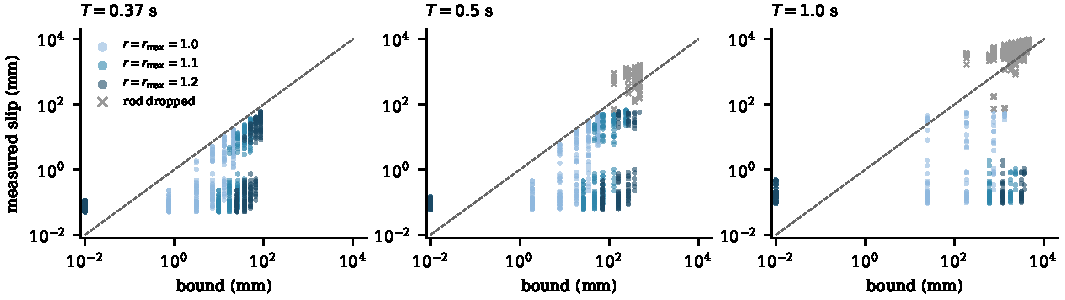
\includegraphics[width=\textwidth]{fig_tightness.pdf}
\caption{\textbf{Bound against measured slip} for deliberately under-gripped lifts (grip 85--100\% of the no-onset grip,
40 objects; log axes, zeros drawn at the left and bottom edges; dashed line: slip equal to the bound). Points below the line
are covered by the bound. Crosses are lifts that dropped the rod, where the slip is the rod's fall.}\label{fig:tightness}
\end{figure*}


